\chapter{Hierarchical Temporal Memory(HTM)}
\section{HTMの概要}
HTMは大脳皮質の構造と学習アルゴリズムを模して作られたニューラルネットワークである。
構造はカラムとセルによる2次元マップ表現となっており、各セルが状態を偏移させる。
学習アルゴリズムはヘブ則となっており各時刻間で活性化状態のセル同士の接続を強める。
また活性化状態のセルと強く接続しているセルが予測状態に遷移することで予測を行う。

HTMは全部にセルを用いて1つのパターンを表現する。各セルの状態が遷移することで表現するパターンが変化する。

HTMの特徴は時系列データ中の各パターンを再現しつつ学習するためオンライン学習を行っているという点とモデルの訓練とデータの再現を同時に行っているという点がある。
これによって時系列データを連続してモデルに流し続け学習を行うという連続オンライン学習が可能となっている。
また疎な分散表現を用いたことによる並列同時予測が可能な点も挙げられる。

\section{HTMの構造}
HTMの全体構造を下の図2.1に示す。
HTMは複数のカラムの集合となっており、各カラムは複数のセルの集合からなっている。
HTM全体で1つのパターンを表現する。時間が進むごとにパターンが変化していくことで時系列データを表現する。

\begin{figure}[ht]
  \begin{center}
    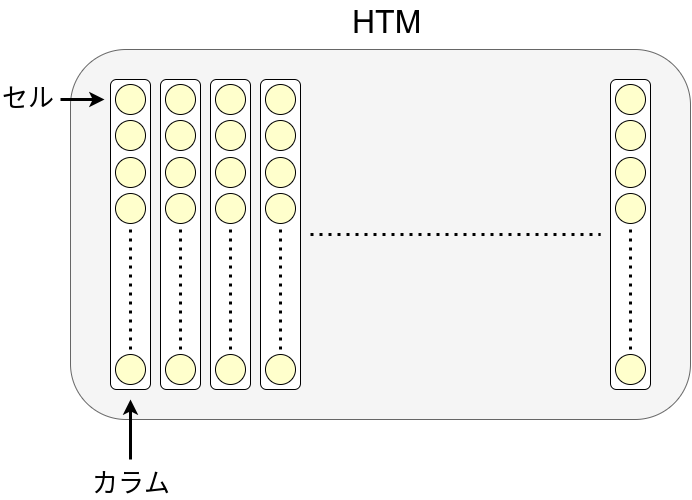
\includegraphics[scale=0.5]{./fig/drawing_1}
    \caption{HTMの全体構造}
    \label{fig:HTM}
  \end{center}
\end{figure}

\subsection{セルの状態変化}
セルの状態は活性化状態と非活性化状態と予測状態の3つであり、各時刻において常にどれか1つの状態を取る。各時刻ごとにそれぞれの状態を相互に遷移する。

\vspace{5mm}
\begin{figure}[ht]
  \begin{center}
    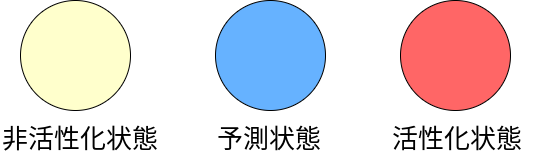
\includegraphics[scale=0.5]{./fig/drawing_2}
    \caption{セルの状態}
    \label{fig:cell_state}
  \end{center}
\end{figure}

\subsection{パターン表現}
HTMはカラムの組み合わせでパターンを表現する。
各カラムにおいてカラム中のセルのどれか1つでも活性化状態になっている場合にそのカラムがパターン表現を構成するカラムとみなす。

\vspace{5mm}
\begin{figure}[ht]
  \begin{center}
    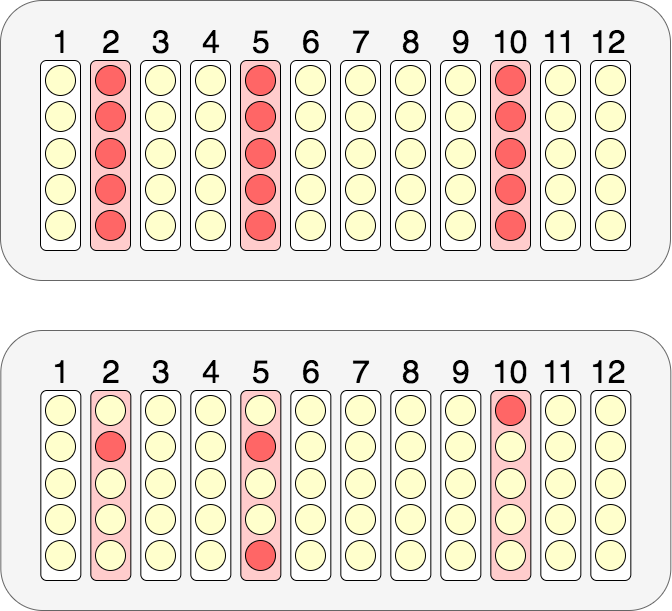
\includegraphics[width=10cm]{./fig/drawing_3}
    \caption{パターンの表現: 上下どちらの図も同じカラムの組み合わせ(2, 5, 10)でパターンを表現しているため、両方同じパターンを表す。}
    \label{fig:pattern_representation}
  \end{center}
\end{figure}

\subsection{セル内の構造}
HTMはセル内にセグメント構造を持っている。
これは大きく分けて2つからなり、入力セグメントとセグメント集合からなる。
入力セグメントは入力を受け取るもので、各セルに1つある。
セグメント集合も各セルに1つあり、接続セグメントを複数持っている。
この接続セグメントは他のセルとの接続値を保持しており、学習によってこの接続値を増減させしきい値との比較によってセル間のシナプス接続を判定する。
接続セグメントはHTM中のすべてのセルとの接続値を持つため2次元のテンソル値となる。
そのためセグメント集合は3次元のテンソル値となる。

\vspace{5mm}
\begin{figure}[ht]
  \begin{center}
    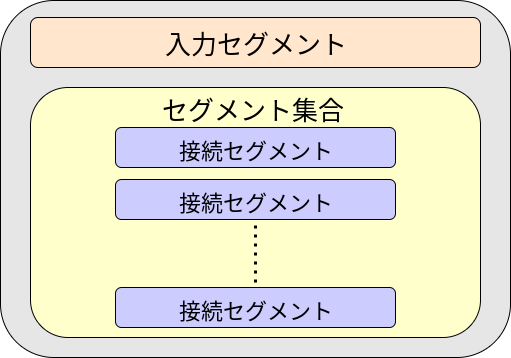
\includegraphics[width=10cm]{./fig/drawing_4}
    \caption{セル内の構造}
    \label{fig:cell_structure}
  \end{center}
\end{figure}

\subsection{疎な分散表現}
学習が進んでいくとHTM中の僅かなセルのみが活性化状態に遷移していき、少ないセルでパターンを表現するようになる。
これによってあるパターンを表現するのに疎な分散表現を用いていると言える。

\section{HTMの学習アルゴリズム}

HTM中のカラムの数を$N$とし、1カラム中のセルの数を$M$とする。
このときHTM中のセルの総数は$M \times N$となる。

活性化状態にあるセルの集合を$M \times N$の2進行列${\bf A}^t$で表し、活性化状態にあるj番目のカラムにあるi番目のセルを$a^t_{ij}$で表す。
同様に予測状態にあるセルの集合を$M \times N$の2進行列${\bf \Pi}^t$で表し、予測状態にあるj番目のカラムにあるi番目のセルを$\pi^t_{ij}$で表す。

各セルにあるセグメント集合の中でd番目のセグメントのj番目のカラムにあるi番目のセルを${\bf D}^d_{ij}$で表す。
またセグメント集合中のセグメントはそれぞれ各セルから他のセルへの接続値を保持しているため、セグメントの接続値がしきい値を超えたセルのみを記録した2進行列${\bf \tilde{D}}^d_{ij}$で接続の可否のみを表す。

入力セグメントに入力を受けたセルが存在するカラムの集合を勝者カラムとし、${\bf W}^t$と表す。

\subsection{活性化状態の計算}
活性化状態の計算は下の式で表される。

\begin{equation}
  a^t_{ij} =
  \left\{
  \begin{alignedat}{3}
    1 \qquad &if \; j\in{\bf W}^t \; and \; \pi^{t-1}_{ij} = 1\\
    1 \qquad &if \; j\in{\bf W}^t \; and \; \sum_i \pi^{t-1}_{ij} = 0\\
    0 \qquad &otherwise
  \end{alignedat}
  \right.
\end{equation}

この式は2つの場合においてセルが活性化状態に遷移することを表している。
1つ目はセルが勝者カラム中のカラムに含まれており、そのセルが予測状態に遷移している場合である。2つ目はセルが勝者カラム中のカラムに含まれており、そのセルを含むカラム中に予測状態に遷移しているセルが1つも存在しない場合である。
図2.3におけるパターンの表現において、上の図は2つ目の条件のみによって活性化状態に遷移した場合で、下の図は1つ目の条件のみによって活性化状態に遷移した場合である。
実際の学習では2つの条件による活性化状態が混在した状態でパターンが表現される。

\subsection{予測状態の計算}
予測状態の計算は下の式で表させる。

\begin{equation}
  \pi^t_{ij} =
  \left\{
  \begin{alignedat}{2}
    1 \qquad &if \; \exists_d\|{\bf \tilde{D}}^d_{ij} \circ {\bf A^t}\|_1 > \theta\\
    0 \qquad &otherwise
  \end{alignedat}
  \right.
\end{equation}

この式はセルが予測状態に遷移する場合を表している。
セグメント集合中のある接続セグメントに関して活性化状態にあるセルとその接続セグメントによって接続しているセルが予測状態に遷移する。
\subsection{セグメント集合を用いた接続値の更新}
セグメント集合が持つ接続値を更新する場合として下の3つの場合が挙げられる。
\begin{itemize}
  \item セルが予測状態になり、その後活性化状態に遷移した場合
  \begin{equation}
    j \in {\bf W}^ t \quad and \quad \exists_{i}(\pi^{t-1}_{ij}) > 0
  \end{equation}

  \item 勝者カラム中にあるどのセルも予測状態になっていなかった場合
  \begin{equation}
    j \in {\bf W}^t \quad and \quad \forall_{i}(\pi^{t-1}_{ij}) = 0
  \end{equation}

  \item セルが予測状態になっていたが、その後活性化状態に遷移しなかった場合
  \begin{equation}
    j \notin {\bf W}^ t \quad and \quad \exists_{i}(\pi^{t-1}_{ij}) > 0
  \end{equation}

\end{itemize}

1つ目と2つ目の場合はシナプス接続を強化する。つまりセグメント集合中にある接続値を増加させる。1つ目の場合はセグメント集合の中ですでに接続値がしきい値を超えている接続セグメントに関して、2つ目の場合はセグメント集合のなかで一番大きい接続値を持つ接続セグメントに関して下の更新式を適用する。

\begin{equation}
  \Delta {\bf D}^d_{ij} = p^+{\bf \dot{D}}^d_{ij} \circ {\bf A}^{t-1} - p^-{\bf \dot{D}}^d_{ij} \circ {\bf (1 - A}^{t-1})
\end{equation}

$p^+$と$p^-$は学習率となっており、$p+$は$p-$より大きい値となっている。

${\bf \dot{D}}^d_{ij}$は${\bf D}^d_{ij}$の正の値をもつ位置のみをとりだした2進行列である。
\begin{equation}
  {\bf \dot{D}}^d_{ij} =
  \left\{
  \begin{alignedat}{2}
    1 \qquad &if \; {\bf D}^d_{ij} > 0\\
    0 \qquad &otherwise
  \end{alignedat}
  \right.
\end{equation}

この更新式は不活性シナプスの接続値を減少させ、活性シナプスの接続値を増加させることによってシナプス接続を強化している。

3つ目の場合はセグメント集合の中でしきい値を超えている接続値を減少させる。これはシナプス接続の減衰を再現している。

\begin{equation}
  \Delta {\bf D}^d_{ij} = p^{--}{\bf \dot{D}}^d_{ij} \; where \; a^t_{ij} = 0 \; and \; \|{\bf \tilde{D}}^d_{ij} \circ {\bf A}^{t-1}\|_1 > \theta \; , \; where \; p^{--} \ll p^-
\end{equation}

\section{HTMの学習の例}

\subsection{学習前}
例として下の図を考える。

\begin{figure}[ht]
  \begin{center}
    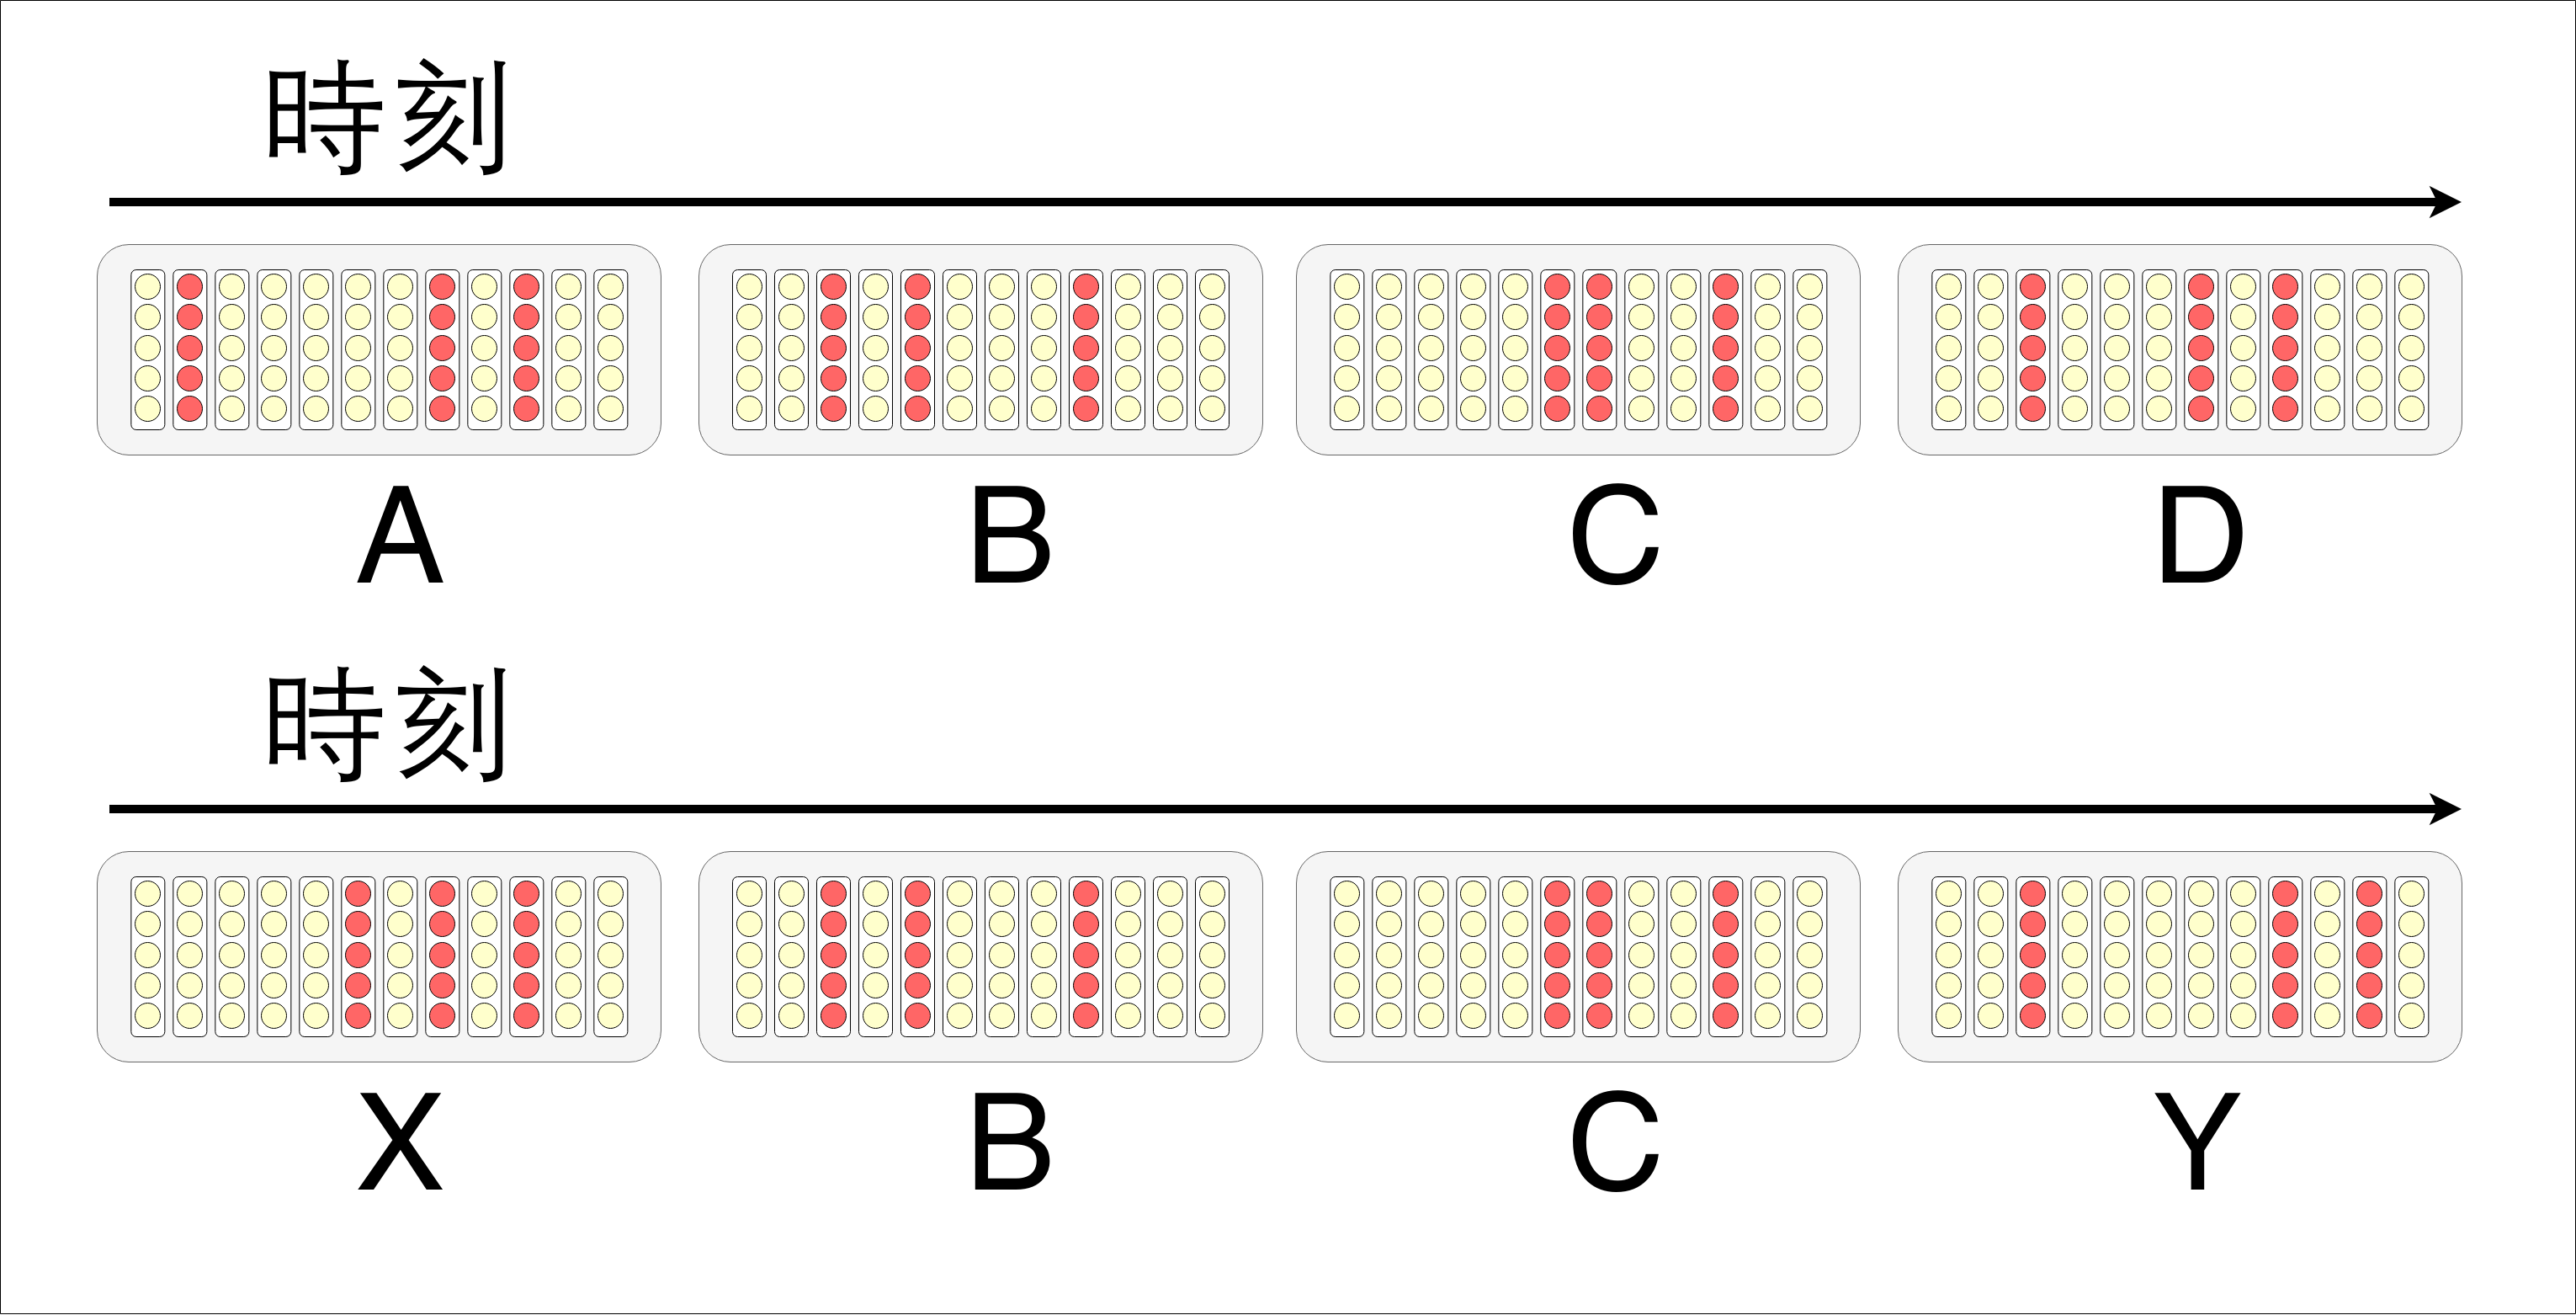
\includegraphics[width=14cm]{./fig/drawing_5}
    \caption{学習前のHTM: (A, B, C, D)という系列と(X, B, C, Y)という系列を入力した場合}
    \label{fig:HTM_before_learning}
  \end{center}
\end{figure}

学習前のHTMは上の図2.5のようになっており、入力に対して予測状態になるセルが存在せずに勝者カラムのセルがすべて活性化状態に遷移していく。

\subsection{学習中}
例として下の図を考える。

\begin{figure}[ht]
  \begin{center}
    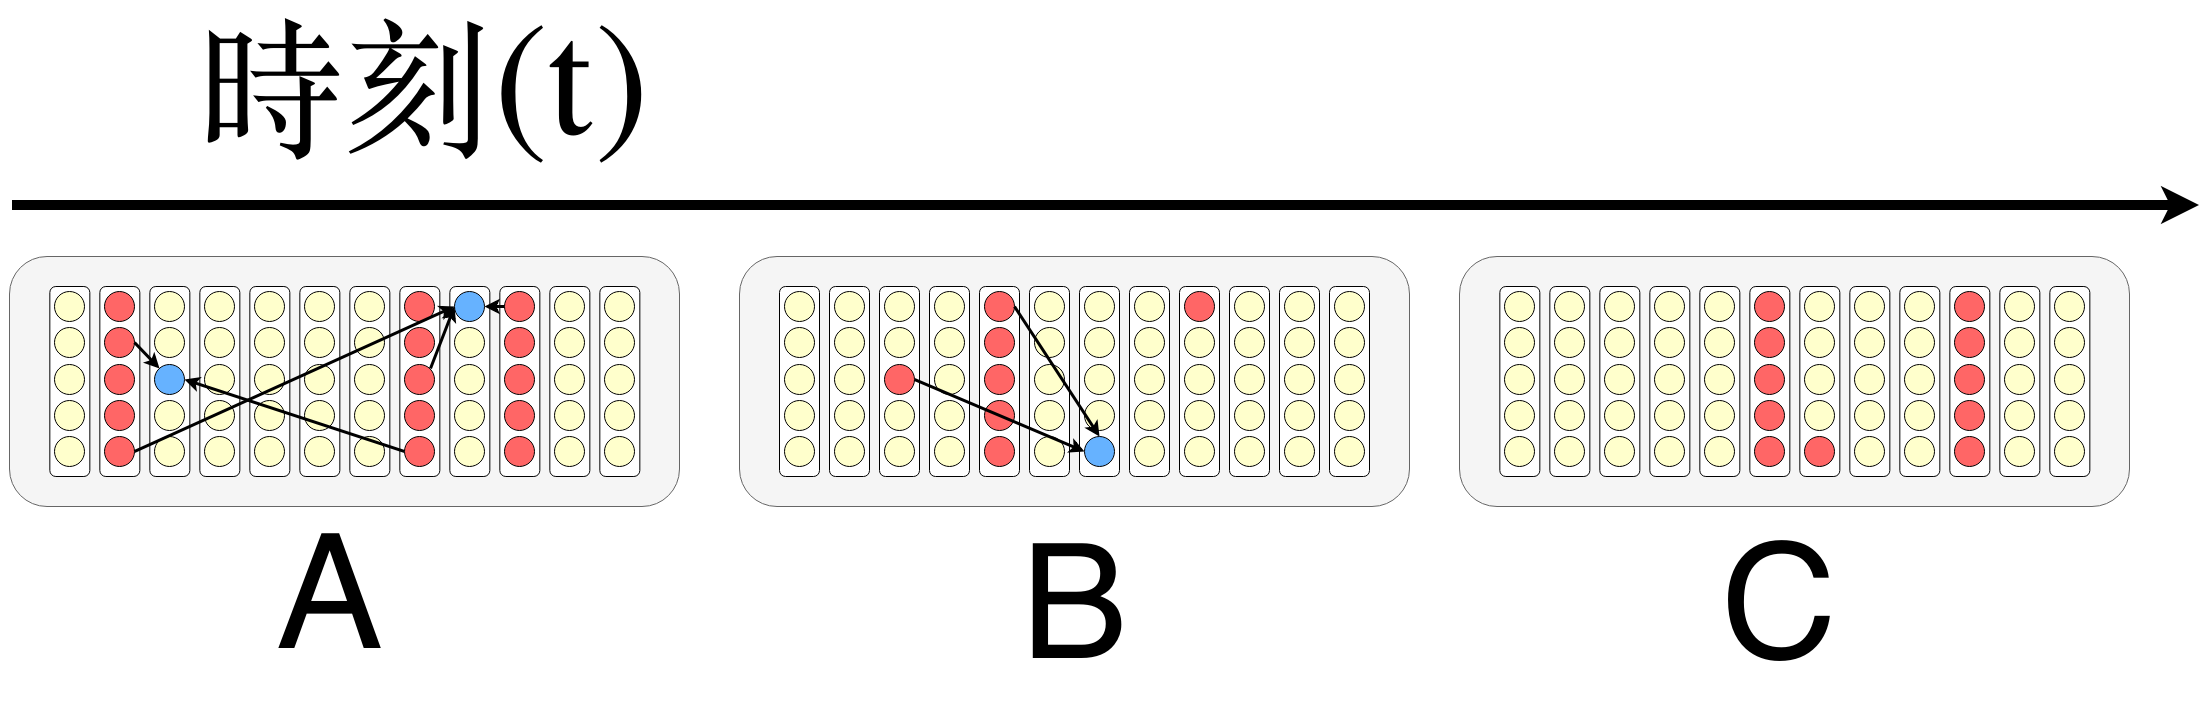
\includegraphics[width=14cm]{./fig/drawing_7}
    \caption{学習中のHTM}
    \label{fig:HTM_during_learning}
  \end{center}
\end{figure}

学習中のHTMは上の図2.6のようになっており、1つ前の時刻の活性化状態のセルとのシナプス結合によってセルが予測状態に遷移することによって次の時刻のパターンが予測される。
また予測状態に遷移するセルが増加するほどパターンの表現が疎になっていく。

\subsection{学習後}
例として下の図を考える。

\begin{figure}[ht]
  \begin{center}
    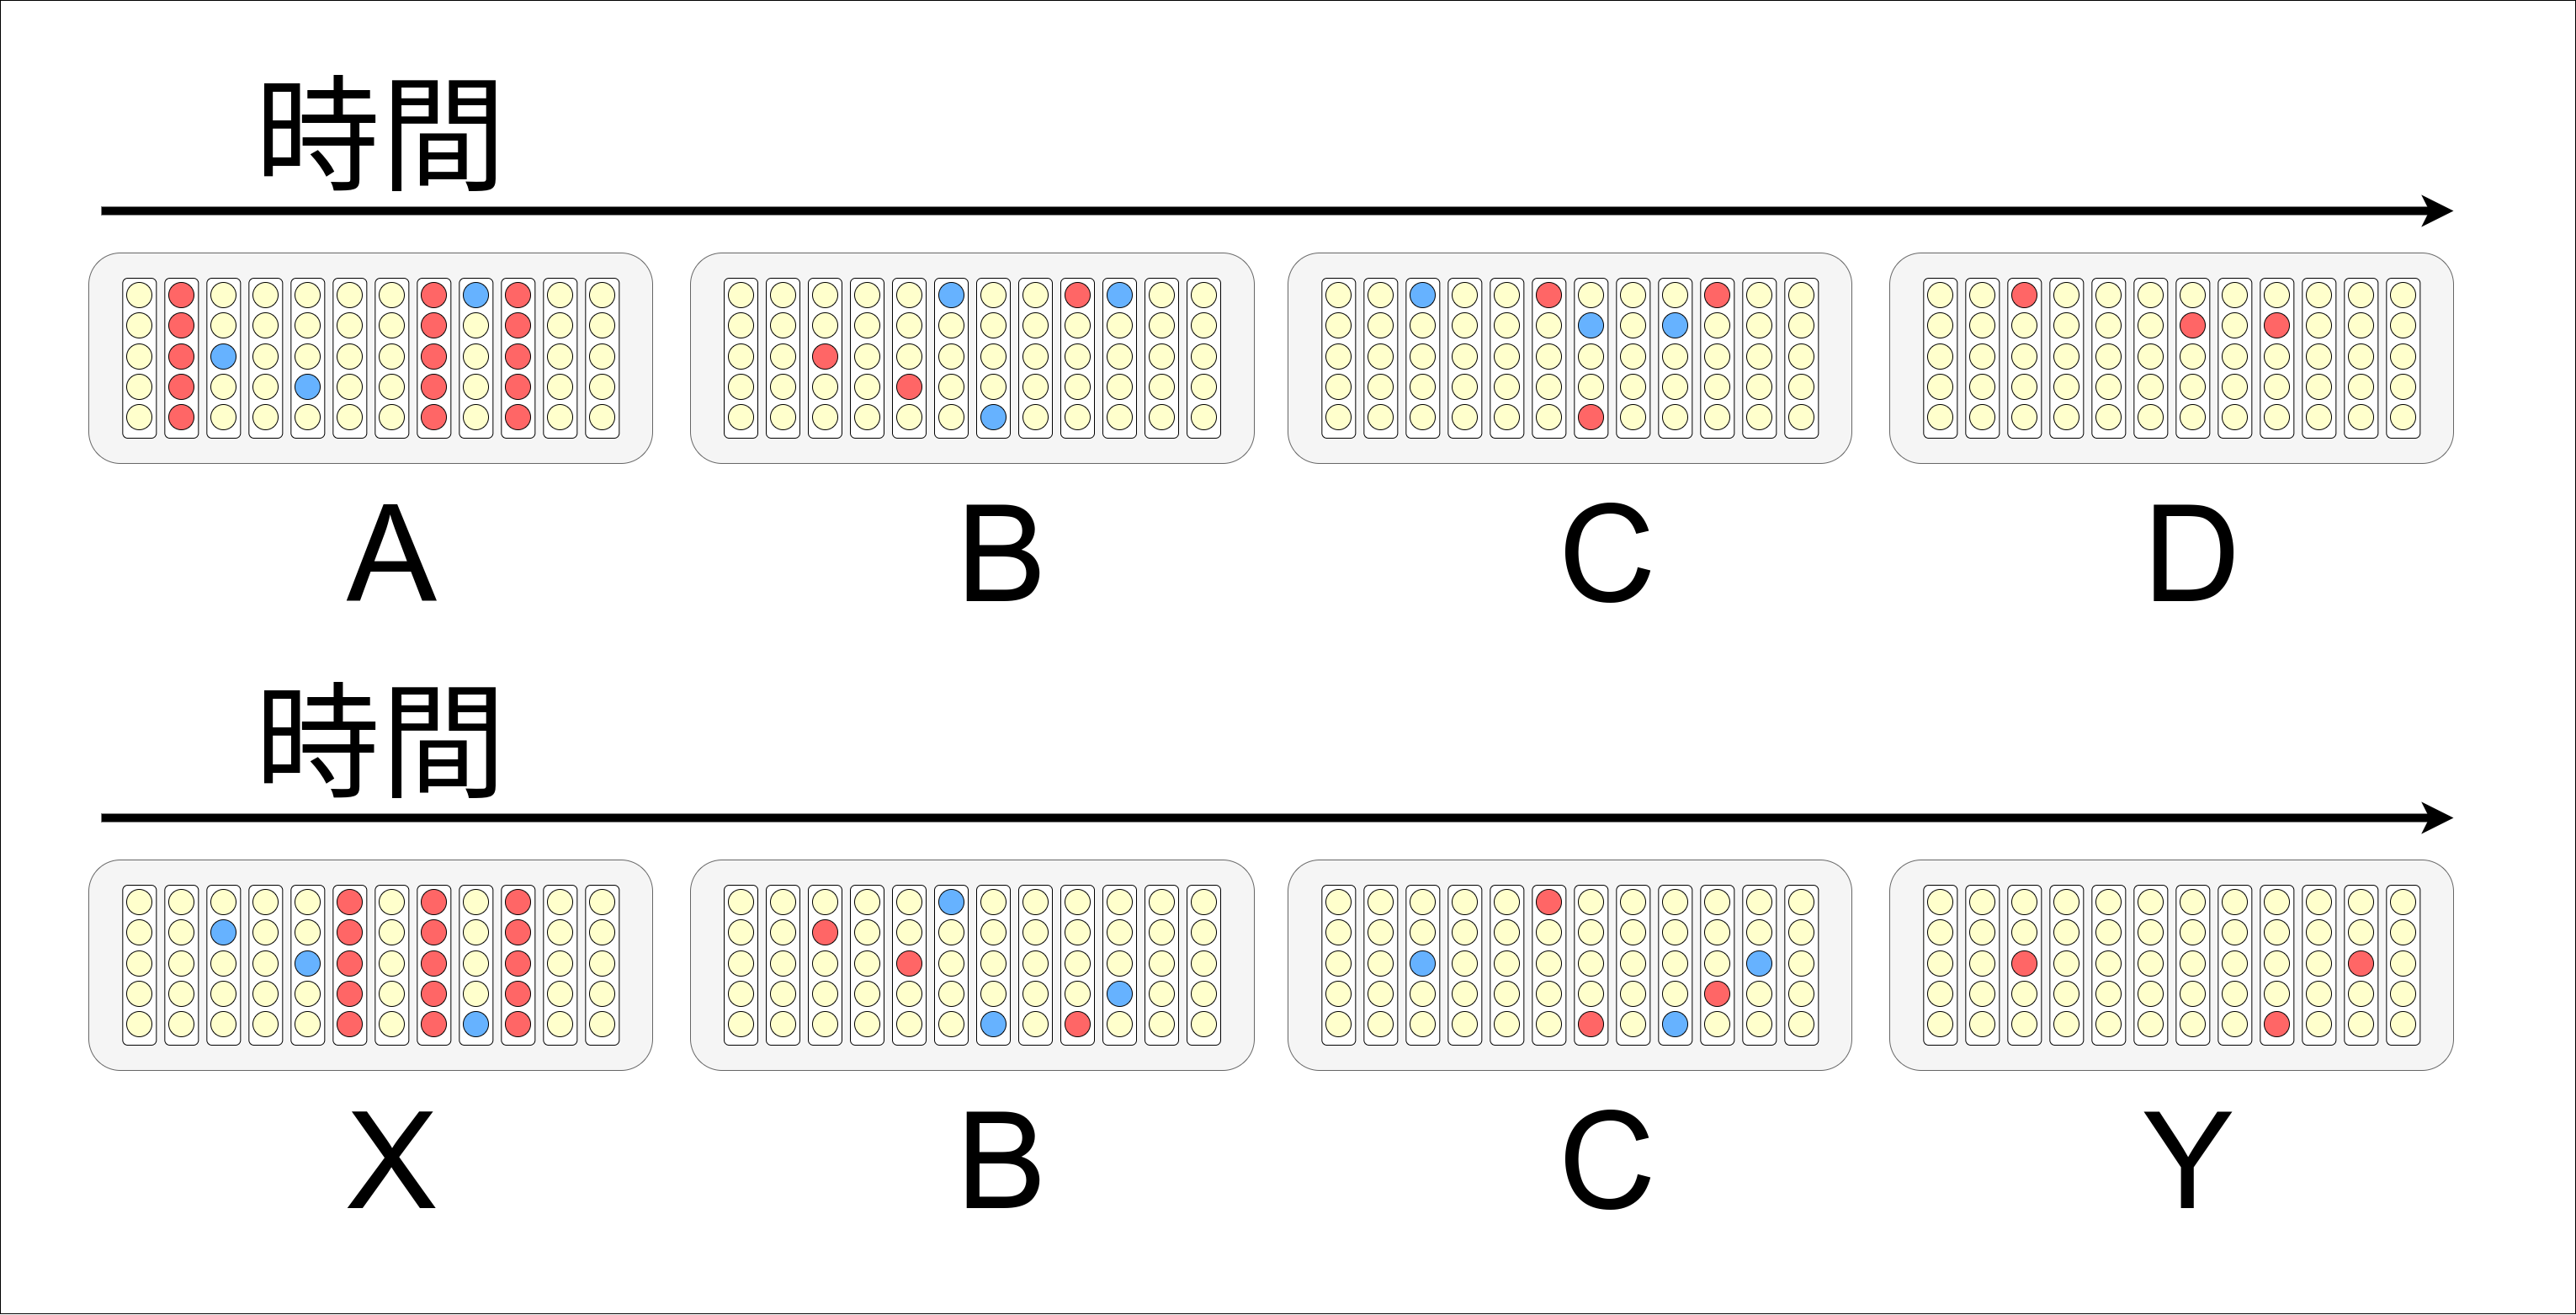
\includegraphics[width=14cm]{./fig/drawing_6}
    \caption{学習後のHTM: (A, B, C, D)という系列と(X, B, C, Y)という系列を入力した場合}
    \label{fig:HTM_after_learning}
  \end{center}
\end{figure}

学習が完了すると最初の入力以外は疎な分散表現によってパターンを表現するようになり、系列中のすべてのパターンが予測されるようになる。

\newpage
\subsection{並列同時予測}

\begin{figure}[ht]
  \begin{center}
    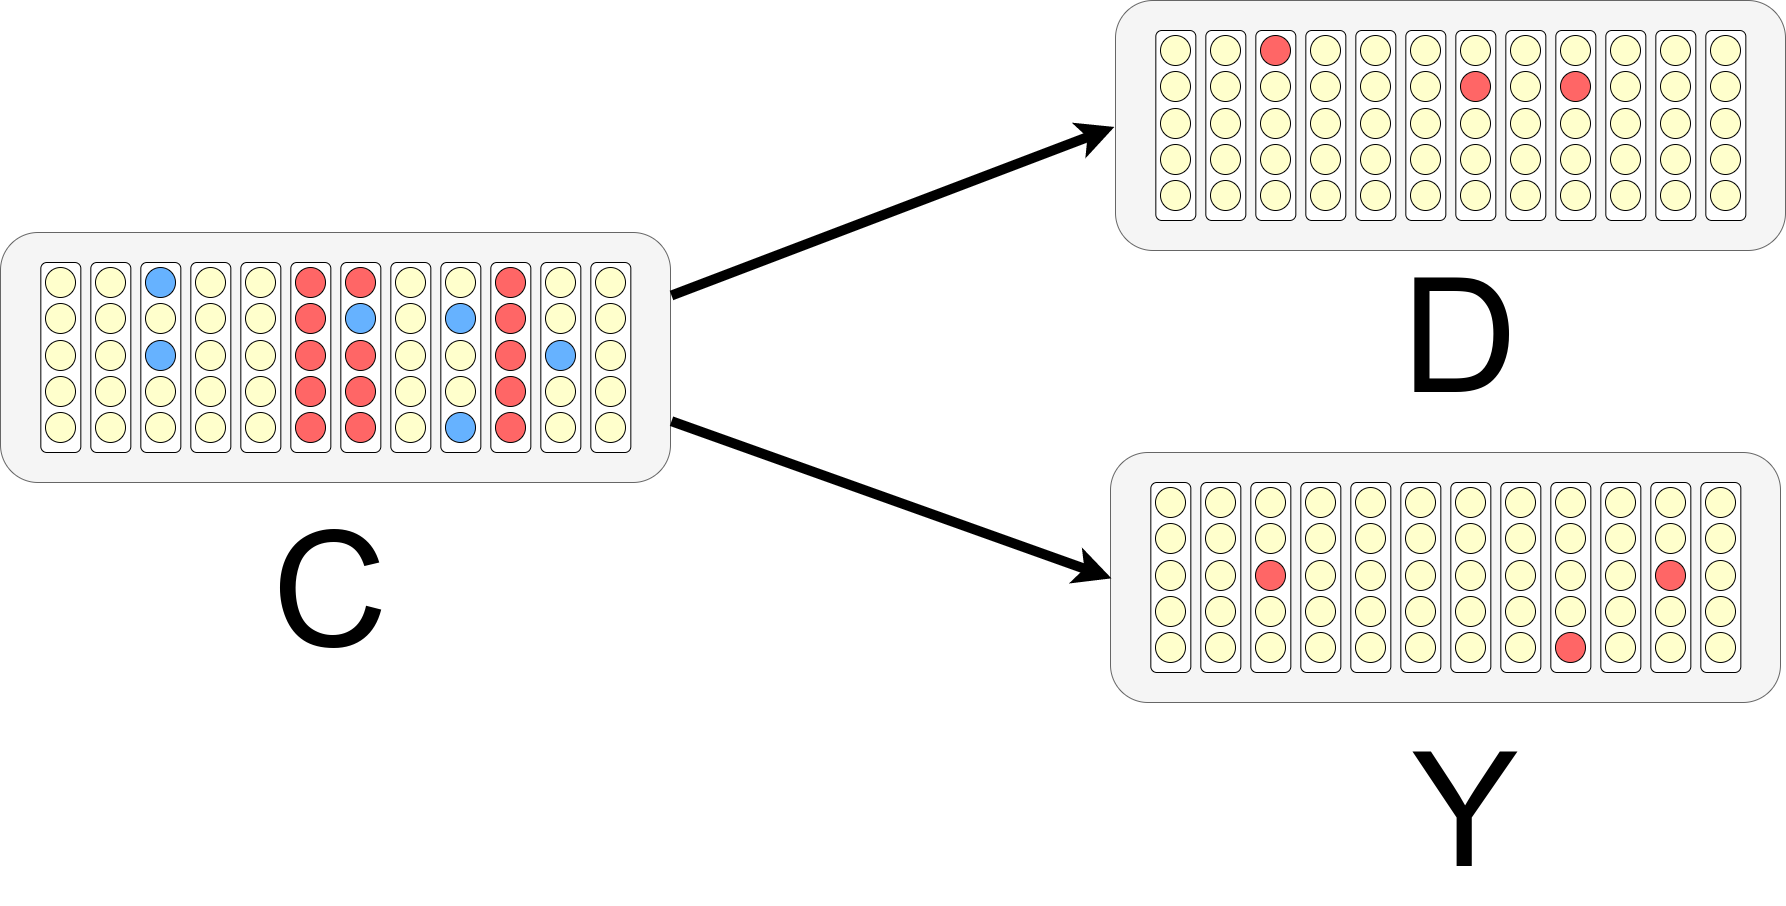
\includegraphics[width=10cm]{./fig/drawing_8}
    \caption{学習後のHTM: (A, B, C, D)という系列と(X, B, C, Y)という系列を学習後に(C)という系列を入力した場合}
    \label{fig:HTM_parallel_prediction}
  \end{center}
\end{figure}

HTMの特徴として並列同時予測が可能であるということが挙げられる。
例として(A, B, C, D)と(X, B, C, Y)という2つの系列を学習後に前の文脈がない状態で(C)という系列を与えたものを考える。
このときCは最初の入力であるため勝者カラムのすべてのセルが活性化状態に遷移する。
これによってDとY両方の予測を導くセルが予測状態に遷移するため、同時に複数の予想が可能になる。

\newpage
\section{エンコーダと分類器}
HTMではパターンの表現はカラムの組み合わせによって表させる。そのためエンコーダによって入力値をカラムの組み合せに変換してHTMに入力し、分類器によってHTMの予測状態のセルから予測されているパターンへ分類することが必要となる。

エンコーダは入力値に対してランダムに一定数のカラムを選び出して割り当てている。
分類器は最尤予測を用いて分類する。HTMの予測状態のセルを以下の式によって各カラムに関する予測点数${\bf P}^t_j$に変換する。

\begin{equation}
  {\bf P}^t_j = \sum^{M}_{i=0} \pi^t_{ij} / M
\end{equation}

${\bf P}^t_j$は長さ$N$の1次行列となる。

ここで各入力値に対応しているカラムの組み合わせをone-hot行列に変換し、${\bf P}^t_j$との要素積をとる。この値をそれぞれの入力に対する予測点数とし、softmax関数に入力することで各入力値に対する予測値を確立分布で出力する。

\section{HTMの問題点}
HTMの問題点は長期依存考慮に関しての性能が低いことがあげられる。
本論文では長期依存考慮の性能を測るために活性化状態の計算に予測状態のセルのみを使用して予測を行った。

\begin{equation}
  a^t_{ij} = \pi^{t-1}_{ij}
\end{equation}

これによってカラムの入力を始めの1つのパターン以外は入れずに、予測状態のみを用いてセルの遷移を行うことになる。
この際に長期依存考慮の性能が低くなる大きな理由として疎な分散表現を用いたことによる2つの問題点がある。
それは以下の2つである。

\begin{itemize}
  \item 疎な分散表現を用いたために発火するセルが徐々に少なくなり消失する。
  \item 学習が大きく進んだパターンにおいて表現が疎になった時に次のパターンに繋がっていたセルが消失するために学習が損失する。
\end{itemize}

1つ目の問題について詳細に述べる。
予測状態のセルの計算によって予測状態にあるセルは疎な分散表現となるが、学習の際は勝者カラムの中でも1つも活性化状態にないときはすべてのセルが活性化状態になることによって予測状態が疎になりすぎることを防いでいた。
しかし長期依存考慮に関する予測タスクでは予測状態のセルのみをもちいて活性化状態を計算するため予測状態になるセルが疎になりすぎてしまい、予測を進める内に予測状態になるセルが消失するという問題が発生した。

2つ目の問題について詳細に述べる。
これは活性化状態の計算によるものであるが、学習が進んでいないときは勝者カラムのほとんどのカラム中のセルすべてが活性化するのに対して、学習が進むにつれて勝者カラムの多くのカラムでカラム中の僅かなセルのみが活性化することになる。これによってその僅かなセル以外とつながっていたセルが予測状態に遷移しなくなるために学習が損失するという問題が発生した。

これらの問題に対処するため、本論文では時間軸セグメントを導入したHTMを提案する。
